\documentclass[conference]{IEEEtran}
\IEEEoverridecommandlockouts
% The preceding line is only needed to identify funding in the first footnote. If that is unneeded, please comment it out.
\usepackage{textcase}
\usepackage{etex}
\usepackage{mathtools}
\usepackage{graphics}
\usepackage{subfigure}
\usepackage{multirow}
\usepackage{fancyhdr}
\usepackage{graphicx}
\usepackage{verbatim}
\usepackage{algorithm,float}
\usepackage{algorithm}
\usepackage{algorithmic}
\usepackage{booktabs}
\usepackage{multirow}
\usepackage{listings}
\usepackage{url}
\usepackage{caption}
\usepackage{epsfig}
\usepackage{epstopdf}
\usepackage{geometry}
\usepackage{pgfplots}
\usepackage{tikz}
\usepackage{amsmath, amsfonts, amssymb, amsthm}
\usepackage{enumerate}
\usepackage{hyperref}
\usepackage{textcomp}
\usepackage{xcolor,colortbl}
\usepackage{array}
\usepackage{cite}
%\usepackage{subfig}
\usepackage{pifont}
\usepackage{pgfplots}
%\pgfplotsset{compat=newest}
\usepgfplotslibrary{groupplots}
\def\BibTeX{{\rm B\kern-.05em{\sc i\kern-.025em b}\kern-.08em
    T\kern-.1667em\lower.7ex\hbox{E}\kern-.125emX}}
\begin{document}

\title{EXPLORING PARALLEL EFFICIENCY AND SYNERGY FOR MAX-P REGION PROBLEM USING PYTHON\\
}

\author{\IEEEauthorblockN{Viney Sindhu}
\IEEEauthorblockA{\textit{Dept. of Computer Science} \\
\textit{Georgia State University}\\
Atlanta, USA \\
vsindhu1@student.gsu.edu}
\and
\IEEEauthorblockN{Danial Aghajarian}
\IEEEauthorblockA{\textit{Dept. of Computer Science} \\
\textit{Georgia State University}\\
Atlanta, USA \\
daghajarian@cs.gsu.edu}
\and
\IEEEauthorblockN{Sushil Prasad}
\IEEEauthorblockA{\textit{Dept. of Computer Science} \\
\textit{Georgia State University}\\
Atlanta, USA \\
sprasad@gsu.edu}
\and
\IEEEauthorblockN{Sergio Rey}
\IEEEauthorblockA{\textit{School of Public Policy} \\
\textit{University of California}\\
Riverside, USA \\
sergio.rey@ucr.edu}}

\maketitle

\begin{abstract}
Given a set of n areas spatially covering a geographical zone such as a
province, forming contiguous regions from homogeneous neighboring areas
satisfying a minimum threshold criteria over each region is an interesting
NP-hard problem that has applications in various domains such as political
science, GIS, etc. In this paper, we focus on a specific case, called the Max-p
regions problem, in which the main objective is to maximize the number of regions while
keeping heterogeneity in each region as small as possible subject to a threshold
constraint. The solution is
broken into two phases. 1) Construction phase: starting from random areas (seeds), the algorithm builds each region by adding neighboring areas to each
growing seed until the region reaches out to the threshold. Then, all the
unassigned regions called enclaves are assigned to their neighboring regions.
2) Optimization phase: tries to improve the feasible solution from phase one by swapping
areas at the border of each region with areas from each neighboring region. In this paper, we
present a parallel implementation of Max-p problem using Python multiprocessing
library. By exploiting a intuitive data structure based on multi-locks, we
achieves up 200-fold and 19-fold speeds up over the best sequential algorithm for
the construction and optimization phases respectively. Also, the overall end to
end running time of our implementation is 35 times faster than this sequential
algorithm. We provide extensive experimental results to verify our algorithm.
\end{abstract}

\begin{IEEEkeywords}
Clustering, Geospatial, Multiprocessing, Optimization
\end{IEEEkeywords}

\section{Introduction}
Clustering geographical areas into homogenous regions has many applications in
various domains such as urban development, districting, transport planning,
analyzing crime rates etc~\cite{r26}. The homogeneous region can be defined as a set
of contiguous areas with high degree of similarity for a given attribute such as
per capita income, population density etc. Generally speaking, problems of this kind are
 NP-hard~\cite{r1} as the size of geographical areas to be
grouped into homogeneous regions increases, the clustering running time
increases exponentially. Hence, it is important to utilize the parallel
processing capabilities of modern hardware to perform the computation. Furthermore, improving the accuracy of the solution by efficiently taking advantage of parallel synergy is another important aspect of these kinds of problems.

Many researchers and scientists have contributed to the problem of aggregating
areas into homogeneous regions. Duque, Anselin, and Rey~\cite{r1} referred to it
as max-p region problem, Hensen~\cite{r2} referred to it as clustering under
connectivity constraints, Maravalle and Simeone~\cite{r3} referred to it as
regional clustering, Wise~\cite{r25} referred to it as regionalization. Major
challenges in solving this problem are to ensure spatial contiguity of each
region, measure homogeneity of each region, explore solution space, and ways to
check solution feasibility. Other constraints in solving this problem are the shape
of the region, equality of an attribute value across the region, and boundary
integrity. Due to these constraints, some different formulations and
solution strategies have been contributed by researchers.

Availability of highly disaggregated spatial data and computational resources
provides the opportunity for researchers to explore new applications of these
clustering models. New opportunities bring new challenges, and one of the
challenges is ever-increasing data size. DiMOS lab, working under the direction of Dr. Prasad, has already laid out the roadmap~\cite{r34,r35} on using GPUs for the parallel processing of geospatial datasets. There are many available algorithms to cluster the areas into homogeneous regions, however, most of them are not
scalable. Another challenge is to decide on the number of homogeneous regions to
be formed after clustering. Most of the available models require the number of
regions as input. Also in order to decide on the best clustering model for a set
of given areas, one needs to know about all the available algorithms. Mostly,
researchers want to design regions for analysis rather than summarizing and
finding the number of regions in the data. In this situation, the researcher may not
know the number of regions to be designed, however they may know the condition
which will make a region suitable for analysis. This information can be used as
criteria to decide the number of regions.

In this paper, we use the clustering model explained in~\cite{r1} as the max-p
problem. The max-p region model is implemented in Python, therefore, to have a benchmark for evaluation of our work, we have also used Python for this research. Another reason to use Python is that lot of researchers are familiar with Python and use it on day to day basis for analysis. 

The problem aggregates $n$ areas into an unknown maximum number of homogeneous regions, where each region satisfies a minimum threshold value for a
given spatial attribute. The problem is formulated as an Integer Linear
Programming (ILP) with a two-part objective function. The algorithm has two
phases: first, it tries to form as many initial regions as possible (the first
part of the objective function) by starting from random areas called seeds and
grow them until each region reaches the threshold. The remaining areas that do
not form regions in the first step are called enclaves and are assigned to their
proximal regions. In the second phase, the algorithm tries to optimize the objective function among those solutions with the maximum number of regions (the second part of the objective function). This goal is achieved by exchanging areas in the border of two neighboring regions. Unlike other models, this model does not impose any constraint on the shape of the regions, instead, the number of regions ($p$) and shape of the regions are data dependent and are decided by the algorithm at runtime. The
max-p model tries to maximize the number of homogeneous regions, based on a predefined minimum threshold value. The degree of aggregation bias is minimized by maximizing the homogeneity within the regions. In this paper, we exploit parallel processing to improve the performance of the max-p model. We also use parallel synergy to improve the accuracy of solutions by trying more solutions in parallel as well as exploiting a fine parallelism model in each solution. Multiple solutions are created simultaneously on multiple processors in parallel and then compared to choose the best feasible solution. Then all the regions of the best feasible solution are processed on multiple processors in parallel to optimize and increase homogeneity within them.

In summary, our key contributions in this work are:
\begin{itemize}

\item Parallel implementation of the construction phase of Max-p problem that is up to 200 times faster than the best sequential algorithm for the largest ($56\times 55$) lattice size.

\item Parallelizing the optimization phase of finding the best feasible solution that is up to 19 times faster than the best sequential algorithm.

\item End to end running time of our parallel implementation achieves 35-fold speed up over the best sequential algorithm for the largest ($56\times 55$) lattice size.

\item Using a parallel data structure based on multiple locks to reduce parallelism overhead.

\item By taking advantage of parallel synergy, we often improve the secondary objective function better then sequential algorithm by exploring the exponential search space in parallel.

\end{itemize}

The rest of the paper is organized as follows. In Section 2, we present literature review. In Section 3, we describe the problem statement. In Section 4, we discuss the algorithm used to solve the problem. In Section 5, we present experimental results and evaluate performance. In Section 6, we summarize the research work.

\section{Literature Review}
In this section, we present a brief survey on various methods of clustering areas into set of homogeneous regions. Algorithm used in one of the methods~\cite{r4, r5} to aggregate areas in to regions has two parts. First part of the algorithm aggregate areas into regions using conventional clustering algorithm. In this part, areas are clustered based on the attributes and not on the locations. In second part of the algorithm, regions are created as subsets of the spatially contiguous areas from the already created clusters. Number of regions created from this method depends on the attributes used to calculate homogeneity within regions~\cite{r7}.

Another method~\cite{r6, r8} uses $x$ and $y$ coordinates of the centroids of
areas as additional attributes in conventional clustering algorithm. Due to
these additional attributes nearby areas will be clustered together. Regions may
not be spatially contiguous, however, contiguity of the areas within the region
depends on the weights assigned to $x$ and $y$ coordinates as compared to other
attributes~\cite{r24}. Increase in weights of $x$ and $y$ coordinates will
increase the spatial contiguity within the regions, however, it will lead to
decrease in weights assigned to other attributes which in turn decreases the
homogeneity within the regions. The main challenge of this method is to decide on how to assign weights to the attributes~\cite{r6, r16, r20}.

There are other methods~\cite{r7, r8, r14, r15, r18} that ensure spatial contiguity based on the information from neighbouring structure. For example, adapted hierarchical clustering algorithms~\cite{r11, r13, r22} allows to merge clusters only if they share common borders. Another example is graph theory based algorithms~\cite{r12, r17, r24} which represents areas and neighbouring structures as connected graphs.

The choice of method to aggregate areas into homogeneous regions depends on the problem. For example, if you want the shape of region to be guided by the spatial distribution of variables, than clustering using $x$ and $y$ coordinate method is not appropriate as it generates circular regions. The method purposed in this article ensures contiguity by clustering only those areas into a region which shares a common border.

\section{Problem Statement}
The main goal of max-p region problem is to cluster the areas into the maximum number of
homogeneous regions such that each region satisfies a predefined minimum
threshold value for a given spatially extensive attribute~\cite{r1}. A spatially extensive
attribute refers to a parameter that we want to be greater than a minimum
threshold for each cluster. For example, in applications of spatial epidemiology
or criminology where the study of rates is the focus, there is a desire to
aggregate areas to ensure that the size of the population at risk (the
denominator of the rate) attains a minimum size to stabilize the variance of the
rate estimates. The second goal of this model is to maximize 
homogeneity within each cluster. In the other words, max-p aims to minimize total
heterogeneity of all clusters. We will define this term later in this section.
The way max-p prioritizes these two goals is that if two clustering
configurations satisfy minimum threshold criteria, the model chooses the one
with the larger number of regions (maximizing p). In case of a tie, the one with less
total heterogeneity is selected.\footnote{The problem statement and equations 3.1 through 3.4 are taken from~\cite{r1}}

\subsection{Preliminary Notation}
The following is the formulation of max-p problem~\cite{r1}.

$Area:$\\
Given n areas $A = \{A_1, A_2, ..., A_n\}$, ($n = |A|$) and m attributes
assigned to each area such that $A_{i,\;y}$ is the y-th attribute of area $A_i$
where $1 \le y \le m$. Also, let $l_i$ denote a parameter that we want to be greater than a minimum
threshold for each region.\\ \\ $Relationship:$\\ Let $d : A \times A \rightarrow R^+ \cup
\{0\}$ be the dissimilarity between areas based on the set of attributes $Y$
such that $d_{ij}\ \equiv \ d(A_i,\ A_j)$ satisfies the conditions $d_{ij}\ \geq
0, d_{ij}\ =\ d_{ji}\ and\ d_{ii}\ =\ 0$ for $i,\ j\ =\ 1,\ 2,\ .\ .\ .\ ,\ n.$
Distance functions can be utilized; i.e., $d_{ij}$ can also satify the
subadditivity, or triangle inequality, condition: $d_{ij} \leq d_{ik}\ +\
d_{kj}$ for $i,\ j,\ k\ =\ 1,\ 2,\ .\ .\ .\ ,\ n.$\\ Let $W\ =\ (V,\ E)$ denote
the contiguity graph associated with A such that vertices $v_i \in V$ correspond
to areas $A_i \in A$ and edges $\{v_i, v_j\} \in E$ if and only if areas $A_i$
and $A_j$ share a common border. \\
 
$Feasible\ Partitions\ of\ A:$\\
Let $P_p = \{R_1,\ R_2,\ ...,\ R_p\}$ denotes a partition of areas $A$ into $p$ regions with $1 \leq p \leq n$ such that:\\
\begin{equation}
\begin{cases}
|R_k|\; >\; 0\; for\; k\; =\;1,\; 2, ...,\;p \\
R_k \cap R_{k'}=\ \theta\ for\ k,\ k'\ =\ 1,\ 2, ...,\ p \wedge k \neq k' \\
\cup_{k=1}^p\ R_k = A\\
\sum_{A_i \in R_k} l_i \geq threshold > 0 for\ k\ =\ 1,2,\ ....,\ p
\end{cases}
\end{equation}

\newcommand{\RNum}[1]{\uppercase\expandafter{\romannumeral #1\relax}}
Let \RNum{2} denotes the set of all feasible partitions of $A$.\\
 \\

We define heterogeneity of a region $R_k$ as Equation~\ref{eq:eq0}:
\begin{equation}\label{eq:eq0}
h(R_k) =\ \sum_{ij:A_i,A_j\in R_k,i\leq j} d_{ij}\\
\end{equation}
where $R_k \in P_p$. We also define total heterogeneity of partition $P_p$ as the sum of heterogeneity over all of its regions (Equation~\ref{eq:eq1}):
\begin{equation}\label{eq:eq1}
H(P_p) =\sum_{k=1}^p h(R_k)
\end{equation}
 
Finally, the max-p problem can be formulated as finding $P_p^* \in \RNum{2}$ such that:

\begin{equation}
\begin{cases}
 |P_p^*| = max(|P_P^*|:P_p \in \RNum{2}) \\
\nexists P_p \in \RNum{2}:|P_p| = |P_p^*| \quad \text{AND}\quad H(P_p) < H(P_p^*) \\
\end{cases}
\end{equation}

Let us illustrate this with a basic example. Table 1 shows a regular lattice
with $n=12$ areas from $A_1$ to $A_{12}$. We consider
two attributes: 1) y is the average income in an area and l is the number of people
in that area where l represents the spatially extensive attribute. The primary
objective is to find the maximum number of contiguous regions. We need to group
these 12 areas in such a way that each region contains at least 100 people (i.e.
threshold = 100). The secondary objective is to find the solution with the
lowest heterogeneity based on attribute y. We used Manhattan distance for
heterogeneity such that $d_{ij}$ = $|y_i - y_j|$.

\newcolumntype{C}[1]{>{\centering\let\newline\\\arraybackslash\hspace{0pt}}m{#1}}

%\onecolumn
\begin{table*}[htb] 
\scriptsize
\begin{tabular}{cc}
\begin{tabular}{|C{2.2cm}|C{2.2cm}|C{2.2cm}|}
\hline
$A_{1}$\newline$y_{1} = 3000,$ $l_{1} = 23$ & $A_{2}$\newline $y_{2} = 3200,$ $ l_{2} = 27$ & $A_{3}$\newline $y_{3} = 3300,$ $ l_{3} = 33$ \\
\hline
$A_{4}$\newline $y_{4} = 5200,$ $ l_{4} = 21$ & $A_{5}$\newline $y_{5} = 5000,$ $ l_{5} = 20$ & $A_{6}$\newline $y_{6} = 3100,$ $ l_{6} = 20$ \\
\hline
$A_{7}$\newline $y_{7} = 5300,$ $ l_{7} = 24$ & $A_{8}$\newline $y_{8} = 5400,$ $ l_{8} = 25$ & $A_{9}$\newline $y_{9} = 5100,$ $ l_{9} = 25$ \\
\hline
$A_{10}$\newline $y_{10} = 7500,$ $ l_{10} = 35$ & $A_{11}$\newline $y_{11} = 7100,$ $ l_{11} = 30$ & $A_{12}$\newline $y_{12} = 7300,$ $ l_{12} = 40$ \\
\hline
\end{tabular}
&
\begin{tabular}{|C{2.2cm}|C{2.2cm}|C{2.2cm}|}
\hline
$A_{1}$\newline $y_{1} = 3000,$ $l_{1} = 23$ & $A_{2}$\newline $y_{2} = 3200,$ $ l_{2} = 27$ & $A_{3}$\newline $y_{3} = 3300,$ $ l_{3} = 33$ \\
\hline
$A_{4}$\newline $y_{4} = 5200,$ $ l_{4} = 21$ & $A_{5}$\newline $y_{5} = 5000,$ $ l_{5} = 20$ & $A_{6}$\newline $y_{6} = 3100,$ $ l_{6} = 20$ \\
\hline
\cellcolor{green!20}$A_{7}$\newline $y_{7} = 5300,$ $ l_{7} = 24$ &\cellcolor{green!20} $A_{8}$\newline $y_{8} = 5400,$ $ l_{8} = 25$ &\cellcolor{green!20} $A_{9}$\newline $y_{9} = 5100,$ $ l_{9} = 25$ \\
\hline
\cellcolor{green!20}$A_{10}$\newline $y_{10} = 7500,$ $ l_{10} = 35$ &\cellcolor{green!20} $A_{11}$\newline $y_{11} = 7100,$ $ l_{11} = 30$ &\cellcolor{green!20} $A_{12}$\newline $y_{12} = 7300$ $ l_{12} = 40$ \\
\hline
\end{tabular}\\
 (a) Input: $n = 12$, $m=2$ & (b) Solution 1: $p=2$, $H=36,500$\\ & \\
\begin{tabular}{|C{2.2cm}|C{2.2cm}|C{2.2cm}|}
\hline
\cellcolor{green!20}$A_{1}$\newline $y_{1} = 3000,$ $l_{1} = 23$ &\cellcolor{blue!20} $A_{2}$\newline $y_{2} = 3200,$ $ l_{2} = 27$ & $A_{3}$\newline $y_{3} = 3300,$ $ l_{3} = 33$ \\
\hline
\cellcolor{green!20}$A_{4}$\newline $y_{4} = 5200,$ $ l_{4} = 21$ &\cellcolor{blue!20} $A_{5}$\newline $y_{5} = 5000,$ $ l_{5} = 20$ & $A_{6}$\newline $y_{6} = 3100,$ $ l_{6} = 20$ \\
\hline
\cellcolor{green!20}$A_{7}$\newline $y_{7} = 5300,$ $ l_{7} = 24$ &\cellcolor{blue!20} $A_{8}$\newline $y_{8} = 5400,$ $ l_{8} = 25$ & $A_{9}$\newline $y_{9} = 5100,$ $ l_{9} = 25$ \\
\hline
\cellcolor{green!20}$A_{10}$\newline $y_{10} = 7500,$ $ l_{10} = 35$ &\cellcolor{blue!20} $A_{11}$\newline $y_{11} = 7100,$ $ l_{11} = 30$ & $A_{12}$\newline $y_{12} = 7300,$ $ l_{12} = 40$ \\
\hline
\end{tabular}
&
\begin{tabular}{|C{2.2cm}|C{2.2cm}|C{2.2cm}|}
\hline
$A_{1}$\newline $y_{1} = 3000,$ $l_{1} = 23$ & $A_{2}$\newline $y_{2} = 3200,$ $ l_{2} = 27$ & $A_{3}$\newline $y_{3} = 3300,$ $ l_{3} = 33$ \\
\hline
\cellcolor{green!20}$A_{4}$\newline $y_{4} = 5200,$ $ l_{4} = 21$ &\cellcolor{green!20} $A_{5}$\newline $y_{5} = 5000,$ $ l_{5} = 20$ & $A_{6}$\newline $y_{6} = 3100,$ $ l_{6} = 20$ \\
\hline
\cellcolor{green!20}$A_{7}$\newline $y_{7} = 5300,$ $ l_{7} = 24$ &\cellcolor{green!20} $A_{8}$\newline $y_{8} = 5400,$ $ l_{8} = 25$ &\cellcolor{green!20} $A_{9}$\newline $y_{9} = 5100,$ $ l_{9} = 25$ \\
\hline
\cellcolor{blue!20}$A_{10}$\newline $y_{10} = 7500,$ $ l_{10} = 35$ &\cellcolor{blue!20} $A_{11}$\newline $y_{11} = 7100,$ $ l_{11} = 30$ &\cellcolor{blue!20} $A_{12}$\newline $y_{12} = 7300,$ $ l_{12} = 40$ \\
\hline
\end{tabular}\\
(c) Solution 2: $p=3$, $H=40,100$ & (d) Solution 3: $p=3$, $H=3,800$\\
\end{tabular}

\caption{An example of max-p problem, (a) input areas, (b) a solution with $p=2$, (c) a feasible solution with $p=3$, (d) another feasible solution with $p=3$. Solution 3 is chosen because it has lowest total heterogeneity among partitions with maximum number of regions ($p=3$).}
\label{tab:tab1}
\end{table*}

As shown in Tables~\ref{tab:tab1}, there are three solutions for partitioning
these areas where Solution 2 and 3 reach the maximum number of regions.
Therefore, Solution 1 is dominated by other solutions with
larger number of regions. Hence, Solution 2 and Solution 3 are the feasible solutions
as we can see that it is not possible to have more than three regions with at
least 100 people per region. Also, we can see that Solution 3 has heterogeneity
lower than that of Solution 2. Therefore, Solution 3 is the best feasible
solution for this example. All the regions of Solution 3 have more than 100
people each. 103 people in $R_{white}$, 115 people in $R_{green}$ and 105 people
in $R_{blue}$.

\section{Methods}
In this section, we present our algorithm to solve the problem of clustering
areas into the maximum number of homogeneous regions. The algorithm has two phases, i.e.
the construction phase and the optimization phase. The construction phase generates a
feasible solution and optimization phase improves the feasible solution by
minimizing the heterogeneity within the regions through local swapping of areas
between neighbouring regions.\footnote{This two phase algorithm is adopted from~\cite{r1}. We extend the Python implementation from~\cite{r1}}

\subsection{Construction Phase}
In this phase, areas are clustered into the maximum number of regions based on
a minimum threshold value of the spatially extensive attribute. An initial feasible
solution is generated at the end of this phase. We repeat this algorithm
multiple times with random seeds (100 times for this experiment) to calculate the set of feasible
solutions. We run this algorithm on multiple processors simultaneously for each
instance to improve the running time of our algorithm. Once all the processes
finish successfully, we compare the output of each process and select the best
feasible solution. We use the objective function explained in~\cite{r1} to
decide on which solution is the best out of all the solutions.

The objective function to be minimized  can be formulated as follows~\cite{r1}.

Parameters:\\
$i$ = index of areas,\\
$k$ = index of regions,\\
$c$ = index of contiguity order (areas are ordered such that areas next to each other share border),\\
$d_{ij}$ = dissimilarity relationship between areas $i$ and $j$ with $i < j$,\\
$[H]$ = Total heterogeneity\\
\begin{equation*}[H]
t_{ij} = \begin{dcases*}
        1,\ if\ area\ i\ and\ j\ belong\ to\ same\ region\ k\\
        0,\ otherwise;
        \end{dcases*}
\end{equation*}
\begin{equation*}[H]
x_i^{kc} = \begin{dcases*}
        1,\ if\ A_i\ is\ assigned\ to\ region\ R_k\ in\ order\ c\\
        0,\ otherwise;
        \end{dcases*}
\end{equation*}
Minimize:
\begin{equation*}[H]
Z = (-\sum_{k=1}^n \sum_{i=1}^n x_i^{k0}) *10^h + \sum_{i} \sum_{j|j>i} d_{ij} t_{ij}
\end{equation*}

The objective function consists of two parts, the first controls the number of
regions and second controls the total heterogeneity $H(P_p)$. The first
part is obtained by adding the number of areas designated as root areas
($X_i^{k0}$), and the second part is obtained by summing the pairwise
dissimilarities between areas assigned to the same region. Since the objective
function is formulated as a minimization problem, we multiply the first term by
minus one.

These two parts are combined together in such a way that there is an implicit
hierarchy where the number of regions comes before the impact of total
heterogeneity. We achieve this hierarchy by multiplying the first term by a
scaling factor $h = 1 + log(\sum_i \sum_{j|j>i} d_{ij})$. For $p$ regions the
objective functions starts at $−p\ast10^h$. This value increases when we add the
total heterogeneity, but $h$ is big enough such that, regardless of the value of
heterogeneity, the objective function will never reach $-(p-1) \ast 10^h$.

\begin{algorithm}
\scriptsize
\caption{: Find best feasible solution~\cite{r1}}
$A$ : set of areas,\\
$l$ : spatially extensive attribute of areas,\\
$W$ : neighborhoods,\\
$t$ : threshold constraint on attribute $l$ at region level,\\
$\Psi$ : set of partitions before enclave assignment,\\
$\epsilon$ : set of enclave areas,\\
$A^u$ : set of unassigned areas,\\
$ns$ : Number of solutions\\
%$p$ : Number of processors\\
\begin{algorithmic}
\vbox{\colorbox{yellow}{\vbox{\STATE \textbf{for} each processor;i = 1 to $ns$ \textbf{do in parallel}}}} 
\begin{ALC@g}
	\WHILE{$A^u \neq empty$}
		\STATE $A_k$ = select at random, one area from $A^u$
		\STATE $A^u = A^u - A_k$
		\STATE $R_k = \{A_k\}$, randomly selected area is assigned to region
		\STATE building\_region = True
		\STATE $T = l_k$, value of attribute $l$ in region $R_k$
		\WHILE{building\_region = True}
			\IF{$T \geq t$}
				\STATE $\Psi = \Psi \cup \{R_k\}$, add region $R_k$ to partition $\Psi$
			\ELSE
				\STATE $N = neighbors \subset A^u$%, set of unassigned-neighbors of all the areas in $R_k$
				\IF{$N \neq empty$}
					\STATE $A_i$ = random area from $N$
					\STATE $A^u = A^u - A_i$
					\STATE $R_k = R_k \cup A_i$
					\STATE $T = T + l_i$
				\ELSE
					\STATE $\epsilon \cup \{R_k\}$
					\STATE building\_region = False
				\ENDIF
			\ENDIF
		\ENDWHILE
	\ENDWHILE
	\IF{$\Psi \neq empty$}
		\STATE feasible = True
		\WHILE{$\epsilon \neq empty$}
			\STATE $\epsilon_i$ = random area from $\epsilon$
			\STATE $\eta$ = region $\eta \subset \Psi $, that shares border with $\epsilon_i$
			\IF{$\eta \neq empty$}
				\STATE $R_k$ = random region $\subset \eta$
				\STATE $R_k^new = R_k \cup \epsilon_i$
				\STATE $\Psi = \Psi - \{R_k\} \cup R_k^new$, update region $R_k in \Psi$
				\STATE $\epsilon = \epsilon - \epsilon_i$
			\ELSE
				\STATE feasible = False
			\ENDIF
		\ENDWHILE
	\ELSE
		\STATE feasible = False
	\ENDIF
\end{ALC@g}
\STATE \textbf{end for}
\STATE $P_{feasible} = \Psi$, at this point all the areas have been assigned to a region
\STATE return $P_{feasible}$
\end{algorithmic}
\end{algorithm}


\begin{algorithm}
\scriptsize
\caption{: Find best feasible solution~\cite{r1}}
$A$ : set of areas,\\
$l$ : spatially extensive attribute of areas,\\
$W$ : neighborhoods,\\
$t$ : threshold constraint on attribute $l$ at region level,\\
$T$ : threshold value
$\Psi$ : set of partitions before enclave assignment,\\
$\epsilon$ : set of enclave areas,\\
$A^u$ : set of unassigned areas,\\
$ns$ : Number of solutions\\
%$p$ : Number of processors\\
\begin{algorithmic}
\vbox{\colorbox{yellow}{\vbox{\STATE \textbf{for} each processor;i = 1 to $ns$ \textbf{do in parallel}}}} 
\begin{ALC@g}
	\WHILE{$A^u \neq empty$}
		\STATE $A_k$ = select at random, one area from $A^u$
		\STATE $A^u = A^u - A_k$
		\STATE $R_k = \{A_k\}$, randomly selected area is assigned to region
		\STATE building\_region = True
		\STATE $T = l_k$, value of attribute $l$ in region $R_k$
		\WHILE{building\_region = True}
			\IF{$T \geq t$}
				\STATE $\Psi = \Psi \cup \{R_k\}$, add region $R_k$ to partition $\Psi$
			\ELSE
				\STATE $N = neighbors \subset A^u$%, set of unassigned-neighbors of all the areas in $R_k$
				\IF{$N \neq empty$}
					\vbox{\colorbox{yellow}{\vbox{\IF {$T - t_{R_k} \geq t_N$}
						\STATE $R_k = R_k \cup N$, add all the neighbours to the region 
						\STATE $A^u = A^u - N$
					\ELSE
						\STATE $A = t_N - (T - t_{R_k})$, select only those many areas which will make region reach minimum threshold value
						\STATE $A^u = A^u - A$
					\ENDIF}}}
					\STATE $T = T + l_i$
				\ELSE
					\STATE $\epsilon \cup \{R_k\}$
					\STATE building\_region = False
				\ENDIF
			\ENDIF
		\ENDWHILE
	\ENDWHILE
	\IF{$\Psi \neq empty$}
		\STATE feasible = True
		\WHILE{$\epsilon \neq empty$}
			\STATE $\epsilon_i$ = random area from $\epsilon$
			\STATE $\eta$ = region $\eta \subset \Psi $, that shares border with $\epsilon_i$
			\IF{$\eta \neq empty$}
				\STATE $R_k$ = random region $\subset \eta$
				\STATE $R_k^new = R_k \cup \epsilon_i$
				\STATE $\Psi = \Psi - \{R_k\} \cup R_k^new$, update region $R_k in \Psi$
				\STATE $\epsilon = \epsilon - \epsilon_i$
			\ELSE
				\STATE feasible = False
			\ENDIF
		\ENDWHILE
	\ELSE
		\STATE feasible = False
	\ENDIF
\end{ALC@g}
\STATE \textbf{end for}
\STATE $P_{feasible} = \Psi$, at this point all the areas have been assigned to a region
\STATE return $P_{feasible}$
\end{algorithmic}
\end{algorithm}

The Construction phase has two different parts: region growing and enclave
assignment.

During region growing a random area is selected from the set of unassigned
areas. Then, this area is added to the region. We check if this newly
formed region reaches the minimum threshold value of the spatial regional attribute.
We stop growing the new region if the minimum threshold value is met, otherwise, we
keep adding unassigned neighbouring areas to the region until it reaches the
minimum threshold value. This is repeated until it is not possible to grow any
new region that satisfies the minimum threshold value. Areas which are not assigned
to any region during growing part are called "enclaves". At the end of growing
part, the algorithm generates set of growing regions and the enclaves are
randomly placed in an enclave queue.

A partial solution generated from growing sub-phase will be processed further by
an enclave assignment step where we pop the enclave queue and attempt to assign
the enclave to a randomly selected neighbouring region. If the selected enclave
is not yet contiguous to an existing region, it is returned to the end of the enclave
queue. The process continues until the enclave queue is exhausted. The algorithm
thus requires that the adjacency graph formed on the areas is connected.

We have tried two different algorithm for construction phase. For the first algorithm, we generate multiple solutions on multiple processes without changing the existing algorithm to generate one solution at a time. For the second algorithm, along with generating multiple solutions on multiple processes, we have also changed the growing part of the algorithm to add multiple neighbours at a time instead of one at a time. Adding multiple areas at a time, helped us to improve the running time of the construction phase of the algorithm.

\subsection{Optimization Phase}
In this phase, the best feasible solution from construction phase is optimized
by minimizing heterogeneity within the regions. We use multiple processors to
perform this task in parallel. Each processor selects a region and all its
neighbours which are eligible to move. Neighbour areas which can be removed from
the region while the region still satisfying minimum threshold value and
contiguity constraint are eligible to move. Each processor acquires two locks,
one on the region where an eligible area is being added and one in the region from
where an eligible area is being moved. Then we move the area which minimizes the
value of objective function. Once the movement is complete, then both the locks
are released and another processor that is ready to move the area from one
region to another can acquire the lock and make the change. This process is
repeated for all the regions in parallel until there is no such neighbour area
which when is moved will further minimize the value of objective function.

\begin{algorithm}
\scriptsize
\caption{: Optimize $P_{feasible}$ to minimize heterogeneity~\cite{r1}}
$A$ : set of areas,\\
$l$ : spatially extensive attribute of areas,\\
$t$ : threshold constraint on attribute $l$ at region level,\\
$\Psi$ : set of partitions,\\
$R$ : set of regions in $\Psi$,\\
$p$ : number of regions
\begin{algorithmic}
\STATE swapping = True
\WHILE{swapping = True}
	\STATE moves = 0\\
	\vbox{\colorbox{yellow}{\vbox{\STATE \textbf{for} each processor: i = 1 to p \textbf{do in parallel}}}}
	\begin{ALC@g}	
		\STATE $R_k$ = random region in $\Psi$
		\STATE $N_{Bk}$ = neighbors of all the areas of region $R_k$
		\STATE \textbf{for} $N_i$ in $N_{Bk}$ \textbf{do}
		\begin{ALC@g}
			\STATE $R_m$ = region that contains neighbor area $N_i$
			\IF{$l_m \geq t$ and doesn't break contiguity}
				\STATE $N_e = N_e \cup N_i$, set of areas which are eligible for movement from region $R_m$ to $R_k$
			\ENDIF
		\end{ALC@g}
		\STATE \textbf{end for}
		\IF{$N_e \neq empty$}
			\STATE $N_{ei}$ = Area from $N_e$ that minimizes the objective function when moved from region $R_m$ to $R_k$
			\IF{$N_{ei} \neq empty$}
					\vbox{\colorbox{yellow}{\vbox{\STATE \textbf{acquire lock on $R_k$ and $R_m$}}}}
				\STATE $R_k = R_k \cup N_{ei}$
				\STATE $R_m = R_m - N_{ei}$
				\STATE move += 1\\
				\vbox{\colorbox{yellow}{\vbox{\STATE \textbf{release lock on $R_k$ and $R_m$}}}}
			\ENDIF
		\ENDIF
	 \end{ALC@g}
	 \STATE \textbf{end for}
	 \IF{moves = 0}
	 	\STATE swapping = False
	 \ENDIF
\ENDWHILE
\STATE $P_p$ = Optimized solution with minimum heterogeneity
\STATE return $P_p$
\end{algorithmic}
\end{algorithm}

First, we find the neighbours of all the areas in a region.  After that, we check for each neighbour that if we remove it from the current region, whether or not the region can maintain its contiguity and also satisfies the minimum threshold criteria. All the neighbour areas which can be removed from the region while the region still satisfying minimum threshold value and contiguity constraint are eligible to move.\\

For each eligible area, we try to move it from its current region to the region assigned to a particular processor. After that, we calculate the objective function value for the new solution and compare it with an already available solution to check if it is smaller than the current value. We take the area which gives us the minimum value of objective function.\\

Once we find the area which minimizes the objective function value, then we acquire the lock on both the regions from which area is being moved and also the region to which area is being moved. We acquire the two locks based on the index of the regions. We acquire the lock first on the region with smaller index and then on the region with the larger index. This is done to avoid the race condition. Once the area is moved, then we release the locks on both the regions. Multiple locks are used to reduce the lock overhead.\\

Let us explain the algorithm with the help of an example. Assume we have the
feasible solutions($P_p$) with three regions.\\

\begin{figure}[h]
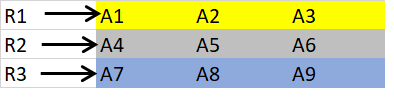
\includegraphics[scale=0.85]{o1.png}
\end{figure}

Region $R_1$, $R_2$ and $R_3$ are sent to processors $P_1$, $P_2$, $P_3$. $P_p$
is a shared memory list which can be updated by all the processors. Now on
processor $P_1$, first we will find all the neighbour areas of $R_1$, which are
eligible to move from their current region. Assume, $N_{R_1}$($A_4, A_5, A_6$) is the list of
neighbour areas which are eligible to move from their current region.\\

\begin{figure}[h]
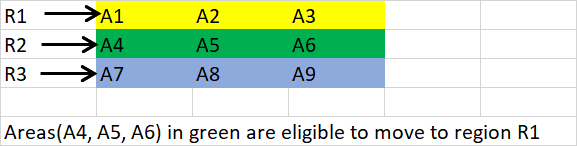
\includegraphics[scale=0.70]{o2.png}
\end{figure}

Now, we will find the area from $N_{R_1}$, which then moving to $R_1$, will
further minimize the objective function. Assume, $A_4$ is the area which
minimizes the current value of objective function. \\

\begin{figure}[h]
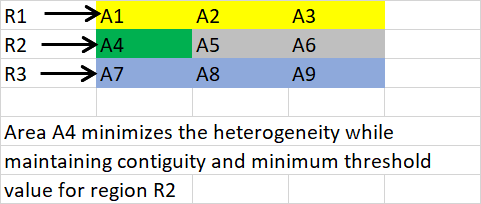
\includegraphics[scale=0.85]{o3.png}
\end{figure}

Processor $P_1$ will acquire lock on region $R_1$ and $R_2$ and move the area $A_4$ from region $R_2$ to
$R_1$. Once, the movement is complete, $P_1$ will release the lock on region $R_1$ and $R_2$. Now, other processors can acquire the lock and update the list. This is repeated on all the processors concurrently. \\

\begin{figure}[h]
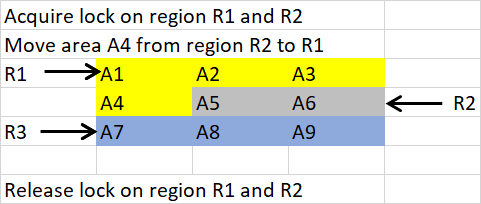
\includegraphics[scale=0.85]{o4.png}
\end{figure}

\footnote{These codes can be downloaded the following link: https://github.com/vineysindhu/parallel-max-p-region.
Also the code for sequential max-p region is available at the following link: https://github.com/pysal}

\section{Experimental Results}
\section{Performance Evaluation}
In this section first, we briefly explain the system we used for our experiments and then presents our results.
\subsection{Experimental Setup}
All the experiments employ a compute node that has 16-core Intel Xeon
CPUE5-2650 V2 CPU running at a clock speed of 2.60 Ghz with 64GB main memory.
All the code for this experiment is written in the Python programming language.
The $multiprocessing$ library available in Python is used to connect to multiple
processors. Also, we have used a compute node that has 64-core AMD Opteron(TM)
Processor 6272 with 64GB main memory for comparison against 16-core Intel.

\subsection{Experiments and Results}

In this section, we evaluate the performance of our algorithm. We have created
regular lattices using $numpy$ library available in Python. Three different sets
of lattices ($20\times 20$, $33\times 33$, $55\times 56$) are created for the
evaluation. We considered two areas to be neighbours if and only if they share a
line (rook). We have also used three different thresholds for spatially
extensive attribute i.e. 25, 100 and 300. We have done several experiments to
evaluate the performance parallel max-p region algorithm. All the experiments are done to explore either the parallel efficiency or the parallel synergy or both in the exponential space. Parallel efficiency means to reduce running time of the algorithm by using parallel processing. Parallel synergy means exploring exponential space by using parallel processing and trying to find the best feasible solution which gives us the minimum value of objective function. Our experiments show that we can achieve both efficiency and synergy by using multiple processes. We have divided the results section further into two parts, Evaluating the efficiency and Exploring synergy.

\subsubsection{Parallel Efficiency:}

We did several experiments to evaluate the performance of our algorithm in terms of running time efficiency. 

\subsubsection*{Average running time comparison of parallel and sequential max-p region algorithm:}
First, we have compared the running time of our algorithm with that of sequential max-p
implementation presented in~\cite{r1}. Table~\ref{tab:tab4} presents the average
running time in seconds for different sets of lattices and different threshold
values for both the sequential and the parallel max-p algorithm. All the timings are taken on Intel 16-core system by using 64 processes for the construction phase and for the optimization phase we have used the number of regions as the number of processes. As shown in table~\ref{tab:tab4}, the speed-up is increasing with lattice size, because smaller lattices form fewer regions. As a result, we are not able to take full advantage of multiprocessing capabilities of the system for small problems. We observed that running time for the optimization phase of a 20x20 lattice for a threshold value of 300 is almost 0, because only one region will be created for $n = 400$ and threshold 300, hence, there will be no optimization phase.

\begin{table*}[!htbp]
\begin{center}
\begin{tabular}{|c|c|c|c|c|c|c|c|c|c|c|}
\hline 
\multirow{2}{*}{Algorithm}&\multirow{2}{*}{Phase} & \multicolumn{3}{|c|}{$20\times 20$} & \multicolumn{3}{|c|}{$33\times33$} & \multicolumn{3}{|c|}{$56\times56$}\\
\cline{3-11}
	& & th=25 & th=100 & th=300  & th=25 & th=100 & th=300  & th=25 & th=100 & th=300\\
\cline{1-11}
\multirow{3}{*}{Sequential Max-p}& Construction  & 10.57& 56.01 & 154.99 & 64.04 & 395.80 &1180.36 &472.89 &3117.80 &9814.39 \\
\cline{2-11}
 & Optimization& 3.33 & 23.28 & 0.01 & 16.46 & 101.64 &774.13 &120.44 &1573.83 &6222.92 \\
\cline{2-11}
 & Total& 13.90 & 79.29 & 155 & 80.50 & 497.44 &1954.49 &593.33 &4691.63 &16037.31\\
\hline
\hline

\multirow{4}{*}{Parallel Max-p}  &Construction& 1.76& 5.68 & 14.86 & 9.29 & 35.18 &104.98 &67.60 &271.32 &829.53\\
\cline{2-11}
 & Optimization& 2.43 & 13.25 & 0.16 & 8.61 & 27.04 &83.36 &29.05 &109.86&320.85 \\
\cline{2-11}
 & Total& 4.19 & 18.93 & 15.02 & 17.90 & 62.22 &188.34 &96.65 &381.18&1150.38 \\
\cline{2-11}
 & Speedup& 3.31 & 4.19 & 10.31 & 4.50 & 7.99 &10.38 &6.14 &12.30 &13.94\\
\hline
\hline

\multirow{4}{*}{New Parallel Max-p} &Construction & 0.54& 0.87 & 1.06 & 2.12 & 3.84 &6.41 &13.55 &25.80&48.88 \\
\cline{2-11}
 & Optimization& 3.61 & 10.85 & 0.17 & 10.64 &23.98 &69.91 &38.24&76.70 & 404.20 \\
\cline{2-11}
 & Total& 4.15 & 11.72 & 1.23 & 12.76 &27.82 &76.32 &51.79 &102.50 & 453.08\\
\cline{2-11}
 & Speedup& 3.35 & 6.76 & 126.02 & 6.31 & 17.88 &25.61 &11.46 &45.77 &35.40\\
\hline
\hline

\multirow{4}{*}{New Sequential Max-p} &Construction & 2.21& 4.31 & 5.95 & 12.80 & 24.39 &40.94 &89.39 &183.14&301.93 \\
\cline{2-11}
 & Optimization& 3.26 & 15.37 & 0.01 & 13.59 & 93.27 &412.92 &94.38 & 754.04 & 3547.81 \\
\cline{2-11}
 & Total& 5.47 & 19.68 & 5.96 & 26.39 & 117.66 &453.86 &183.77 &937.18 &3849.74\\
\cline{2-11}
 & Speedup& 2.54 & 4.03 & 26.01 & 3.05 & 4.23 &4.31 &3.23 &5.01 &4.17\\
\hline

\end{tabular}
\caption{Average running time comparison for three different thresholds(th = Threshold)}
\label{tab:tab4}
\end{center}
\end{table*}

\subsubsection*{Average running time comparison of the construction phase of parallel max-p
region on 16-core Intel processor to that of 64-core AMD Opteron processor:}
We have also compared the running time of the construction phase of parallel max-p
region on 16-core Intel processor to that of 64-core AMD Opteron processor. This
comparison is done for two lattices 20x20 and 55x56 with a threshold of 100 and
300 by using the different number of processes to find best feasible solution i.e.
8, 16, 32, 64, 128, 256, 512. Figure~\ref{plt:plt1} presents the charts which
show that running time of algorithm decreases with increase in the number of
processes up to a certain limit and after that, it starts to increase again. It can
be interpreted from the graph that for 16-core Interprocessor threshold to
decrease running time is 64 and for 64-core AMD Opteron threshold is 128. Once
this threshold is reached, running starts to increase again. Hence, it is clear
from the results that we should use 64 processes for 16-core Intel system and
128 processes for 64-core AMD system to get the best running time. We also
analysed the CPU usage for each process for the different number of processes. For
16-core Intel system, each process can utilize 100 percent of CPU
capacity for up to 16 processes and after that, it decreases to 50 percent for 32
processes. It becomes stable at 17 percent after 128 processes. For 64-core AMD
system, each process can utilize 100 percent of CPU capacity for up to 64
processes and starts decreasing after that. It becomes stable at 70 percent
after 128 processes.

\begin{figure*}[!htbp] 
\centering
\footnotesize
\captionsetup{justification=centering,font=scriptsize,labelfont=scriptsize}
\begin{tikzpicture}

\begin{groupplot}[group style={group name=timeplots, group size=4 by 1, vertical sep=50pt},]
	
	% (1) Construction_20_by_20_100
        \nextgroupplot[ title=\scriptsize{\it{(a) Construction, $20\times 20$, T=100}},                
        legend style={font=\scriptsize\selectfont, at={(.5,.5)}},   
        legend to name={CommonLegend},
	width=5cm,
	xtick=data,
	xlabel=\scriptsize{Number of processes},	
	ylabel=\scriptsize{Construction Time (Second)},	
	ticklabel style={font=\tiny},
	ybar=2pt,
	bar width=4,
	symbolic x coords={8, 16, 32, 64, 128, 256, 512},
	legend style={at={(0.5,-0.15)},
	anchor=north,legend columns=-1},]
	\addplot %C16
	coordinates {(8, 19.7566924) (16, 10.1574373) (32, 8.69590521) (64, 8.68785) (128, 8.69443035) (256, 9.19689488)  (512, 11.0752358)};
	\addplot %C64
	coordinates {(8, 25.22938681) (16, 13.21703243) (32, 8.191967964) (64, 5.847429514) (128, 5.593388081) (256, 6.479811192)  (512, 9.207715988)};	
		
	% (2) Construction_20_by_20_300
        \nextgroupplot[ title=\scriptsize{\it{(b) Construction, $20\times 20$, T=300}},                
	width=5cm,
	xtick=data,
	xlabel=\scriptsize{Number of processes},	
	ticklabel style={font=\tiny},
	ybar=2pt,
	bar width=4,
	symbolic x coords={8, 16, 32, 64, 128, 256, 512},
	legend style={at={(0.5,-0.15)},
	anchor=north,legend columns=-1},]
	\addplot %C16
	coordinates {(8, 54.3102264) (16, 27.9825938) (32, 23.5189321) (64, 22.9158623) (128, 22.704982) (256, 23.2577519)  (512, 25.2306385)};
	\addplot %C64
	coordinates {(8, 73.19414949) (16, 37.92048073) (32, 22.34558034) (64, 15.314605) (128, 13.84061956) (256, 14.93554544)  (512, 17.71974301)};			
	%\legend{\footnotesize{16 Cores},\footnotesize{64 Cores}}
	% (3) Construction_55_by_56_100
        \nextgroupplot[ title=\scriptsize{\it{(c) Construction, $55\times 56$, T=100}},                
	width=5cm,
	xtick=data,
	xlabel=\scriptsize{Number of processes},	
	ticklabel style={font=\tiny},
	ybar=2pt,
	bar width=4,
	symbolic x coords={8, 16, 32, 64, 128, 256, 512},
	legend style={at={(0.5,-0.15)},
	anchor=north,legend columns=-1},]
	\addplot %C16
	coordinates {(8, 1077.90734) (16, 548.340364) (32, 482.395232) (64, 441.882966) (128, 443.576337) (256, 445.830552)  (512, 450.111493)};
	\addplot %C64
	coordinates {(8, 1383.2089) (16, 717.1080742) (32, 404.3155475) (64, 266.8883119) (128, 242.9845831) (256, 245.6331537)  (512, 251.886045)};			
		
	% (4) Construction_55_by_56_300
        \nextgroupplot[ title=\scriptsize{\it{(d) Construction, $55\times 56$, T=300}},                
	width=5cm,
	xtick=data,
	xlabel=\scriptsize{Number of processes},	
	ticklabel style={font=\tiny},
	ybar=2pt,
	bar width=4,
	symbolic x coords={8, 16, 32, 64, 128, 256, 512},
	legend style={at={(0.5,-0.15)},
	anchor=north,legend columns=-1},]
	\addplot %C16
	coordinates {(8, 3314.79092) (16, 1683.59453) (32, 1484.0552) (64, 1347.91893) (128, 1351.03222) (256, 1353.39058)  (512, 1362.93501)};
	\addplot %C64
	coordinates {(8, 4120.620288) (16, 2174.580753) (32, 1234.789869) (64, 807.8640451) (128, 725.6319218) (256, 733.2447016)  (512, 748.6452534)};	
	
      \end{groupplot}
      \path ( $(timeplots c2r1.south east)!0.5!(timeplots c3r1.south west)$) -- node[below]{\ref{CommonLegend}} ($(timeplots c2r1.south east)!0.5!(timeplots c3r1.south west)$);
    \end{tikzpicture}
    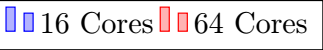
\includegraphics[scale=0.50]{legend.png}
    \caption{Average running time of construction phase on 16-core Intel vs 64-core AMD Opteron}
    \label{plt:plt1}
  \end{figure*}

\begin{figure}[h]
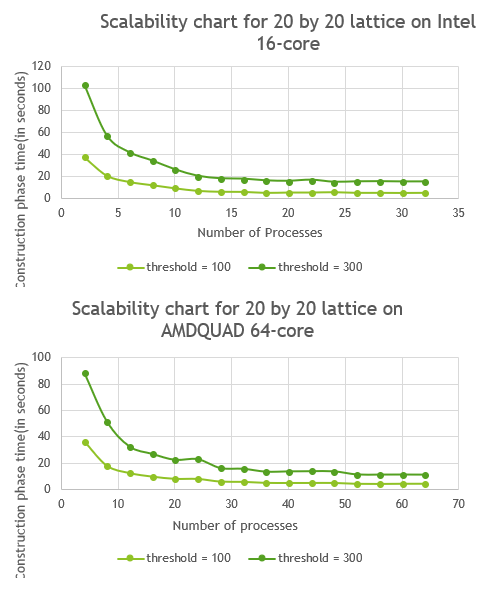
\includegraphics[scale=0.85]{scale20.png}
\end{figure}

\begin{figure}[h]
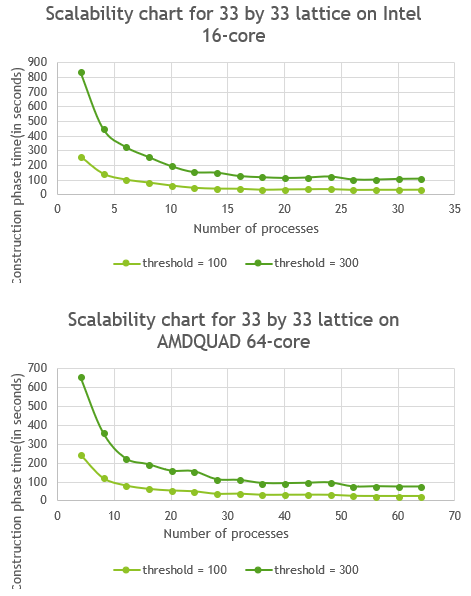
\includegraphics[scale=0.85]{scale33.png}
\end{figure}

\subsubsection*{Single lock vs multiple locks average running time comparison of the optimization phase:}
We started by using single lock on the list of regions in optimization phase.
This lead to a lock overhead problem. In order to reduce the lock overhead, we have
used multiple locks i.e. one lock for each region. After using multiple locks,
we can reduce lock overhead time. Table~\ref{tab:tab5} presents the
running time of the optimization phase for different lattices and different
thresholds. It can be seen that after using multiple locks, the running time of the algorithm is reduced.

\begin{table*}[!htbp] 
\begin{center}
\begin{tabular}{|C{1.4cm}|C{1.4cm}|C{1.4cm}|C{1.4cm}|C{1.4cm}|}
\hline
Lattice & \multicolumn{2}{|c|}{threshold = 100} & \multicolumn{2}{|c|}{threshold = 300}\\
\hline
& Single Lock & Multiple Locks & Single Lock & Multiple Locks\\
\hline
20x20\newline(n = 400) & 17.47 & 13.25 & 0.29 & 0.16\\
\hline
33x33\newline(n = 1,056) & 41.53 & 27.04 & 133.76 & 83.36\\
\hline
55x56\newline(n = 3,080) & 156.47 & 109.86 & 639.63 & 320.85\\
\hline
\end{tabular}
\caption{Single lock vs multiple locks average running time for optimization phase in seconds}
\label{tab:tab5}
\end{center}
\end{table*}

\subsubsection*{Relation between number of areas moved and decrease in objective function value:}
We have also analysed the effect of movement of areas from one region to another on
objective function value. The decrease in objective function value is directly
proportional to the movement of areas from one region to another in each
iteration of optimization phase. More areas moving from one region to another
decreases the value of the objective function. Table~\ref{tab:tab6} presents
the decrease in objective function value with the increase in the number of areas
moved from one region to another. There are few outliers also, for example in
iteration 3 number of areas moved decreased while the objective
function value increased.

\begin{table*}[!htbp]
\begin{center}
\begin{tabular}{|C{1.4cm}|C{1.4cm}|C{1.4cm}|C{1.4cm}|}
\hline
Iteration & Number of areas moved & Decrease in Objective Function Value & Percentage Decrease\\
\hline
1 & 12 & 1.59 & 0.026\\
\hline
2 & 12 & 1.58 & 0.026\\
\hline
3 & 11 & 1.62 & 0.028\\
\hline
4 & 11 & 1.14 & 0.020\\
\hline
5 & 10 & 0.94 & 0.017\\
\hline
6 & 11 & 1.38 & 0.025\\
\hline
7 & 10 & 0.63 & 0.012\\
\hline
8 & 7 & 0.29 & 0.005\\
\hline
9 & 6 & 0.54 & 0.010\\
\hline
10 & 4 & 0.15 & 0.003\\
\hline
11 & 2 & 0.19 & 0.004\\
\hline
12 & 4 & 0.25 & 0.005\\
\hline
13 & 4 & 0.09 & 0.002\\
\hline
14 & 1 & 0.004 & 0.000\\
\hline
15 & 1 & 0.004 & 0.000\\
\hline
16 & 0 & 0 & 0.000\\
\hline
\end{tabular}
\caption{Decrease in objective function value with the decrease in areas moved in optimization phase for 20x20 lattice with threshold = 25}
\label{tab:tab6}
\end{center}
\end{table*}

Since we are doing the filtering of the list of areas and regions multiple times in our code, we decided to run a small experiment to explore various methods to filter the list and see which one gives the best performance. We tried the below methods and found that list compression method is the fastest of all the methods to filter the Python lists.

Running time using set(a) - set(b) : 2.86102294921875e-06 seconds\\
Code - list(set(neighbors)-set(enclaves))

Running time using list compression : 2.384185791015625e-06 seconds\\
Code - [neighbor for neighbor in neighbors if neighbor not in enclaves]

Running time using One of the lists as set : 3.337860107421875e-06 seconds\\
Code - [neighbor for neighbor in neighbors if neighbor not in set(enclaves)]

Running time using lambda function : 5.0067901611328125e-06 seconds\\
Code - list(filter(lambda x: x not in set(enclaves), neighbors))

\subsubsection{Exploring synergy or accuracy of the parallel max-p region algorithm:}

We did the following experiments to explore the synergy of the parallel max-p region algorithm. 

\subsubsection*{Analysis of top solutions after the construction phase:}
First, we analysed the top feasible solutions obtained after construction phase of the algorithm. Table ~\ref{tab:tab8}, ~\ref{tab:tab9} and ~\ref{tab:tab10} presents the analysis for 20x20, 33x33 and 55x56 lattices with threshold 25 respectively. All the solutions present in the tables give the maximum number of regions for their respective lattice size. We can see from the table ~\ref{tab:tab8} that our algorithm will select the solution with minimum objective function value after construction phase and tries to optimize it. Hence, Solution 1 will be chosen for optimization. However, when we analysed other top solutions, we found that Solution 5, does not have minimum objective function value after construction phase, but it gives us best results after optimization phase. Similarly, in the table ~\ref{tab:tab9}, Solution 3 gives the best results after optimization, however, it will not be selected at first by the algorithm. Also, in the table ~\ref{tab:tab10}, Solution 5 gives the best results.

\begin{table*}[!htbp] 
\begin{center}
\begin{tabular}{|C{1.4cm}|C{1.4cm}|C{1.4cm}|}
\hline
Solutions & Objective function\newline value after \newline construction phase & Objective function\newline value after\newline optimization phase\\
\hline
Solution 1 & 63.13 & 54.28\\
\hline
Solution 2 & 63.92 & 54.14\\
\hline
Solution 3 & 63.27 & 54.89\\
\hline
Solution 4 & 63.60 & 55.93\\
\hline
Solution 5 & 63.32 & 51.49\\
\hline
\end{tabular}
\caption{Exploring synergy in top solutions for 20x20 lattice with threshold = 25}
\label{tab:tab8}
\end{center}
\end{table*}

\begin{table*}[!htbp] 
\begin{center}
\begin{tabular}{|C{1.4cm}|C{1.4cm}|C{1.4cm}|}
\hline
Solutions & Objective function\newline value after \newline construction phase & Objective function\newline value after\newline optimization phase\\
\hline
Solution 1 & 173.94 & 148.38\\
\hline
Solution 2 & 173.72 & 148.36\\
\hline
Solution 3 & 174.49 & 145.25\\
\hline
Solution 4 & 174.39 & 151.35\\
\hline
\end{tabular}
\caption{Exploring synergy in top solutions for 33x33 lattice with threshold = 25}
\label{tab:tab9}
\end{center}
\end{table*}

\begin{table}[!htbp]
\begin{center}
\begin{tabular}{|C{1.4cm}|C{1.4cm}|C{1.4cm}|}
\hline
Solutions & Objective function\newline value after \newline construction phase & Objective function\newline value after\newline optimization phase\\
\hline
Solution 1 & 498.15 & 410.82\\
\hline
Solution 2 & 493.82 & 411.39\\
\hline
Solution 3 & 497.09 & 413.88\\
\hline
Solution 4 & 497.88 & 415.94\\
\hline
Solution 5 & 497.51 & 408.86\\
\hline
\end{tabular}
\caption{Exploring synergy in top solutions for 55x56 lattice with threshold = 25}
\label{tab:tab10}
\end{center}
\end{table}

\subsubsection*{Comparison of change in objective function value of sequential and parallel max-p region algorithm:}
We have also analysed the change in objective function value during optimization
phase and its relation to the number of areas moved from one region to another.
Table~\ref{tab:tab7} presents the change in objective function value and the number
of areas moved in optimization phase for both sequential max-p and parallel
max-p algorithm. As shown in table ~\ref{tab:tab7}, the decrease in objective
function value is directly proportional to the number of areas moved from one
region to another. The parallel max-p algorithm can perform similarly to
the sequential max-p algorithm in terms of decrease in the objective function
value. However, there are few outliers where sequential max-p algorithm performs
much better than the parallel max-p.

\begin{table*}[!htbp]
\begin{center}
\begin{tabular}{|c|c|c|c|c|c|c|c|c|c|c|}
\hline 
\multirow{2}{*}{Algorithm}&\multirow{2}{*}{Phase} & \multicolumn{3}{|c|}{$20\times 20$} & \multicolumn{3}{|c|}{$33\times33$} & \multicolumn{3}{|c|}{$56\times56$}\\
\cline{3-11}
	& & th=25 & th=100 & th=300  & th=25 & th=100 & th=300  & th=25 & th=100 & th=300\\
\cline{1-11}
\multirow{3}{*}{Sequential Max-p}& Initial  & 61.99& 64.10 & 64.82 & 172.68 & 177.21 &178.41 &495.41 &507.28 &510.42 \\
\cline{2-11}
 & Final& 50.64 & 58.21 & 64.82 & 141.00 & 160.73 &165.95 &409.91 &439.13 &461.91 \\
\cline{2-11}
 & Decrease& 11.35 & 5.89 & 0.00 & 31.68 & 16.48 &12.46 &85.50 &68.15 &48.51\\
\cline{2-11}
 & Areas Moved& 130 & 79 & 0 & 388 & 245 &219 &1069 &1022 &745\\
\hline
\hline

\multirow{4}{*}{Parallel Max-p}  &Initial  & 62.05& 63.78 & 64.82 & 172.71 & 177.40 &187.34 &494.98 &508.21 &511.75 \\
\cline{2-11}
 & Final& 51.15 & 57.41 & 64.82 & 145.25 & 157.44 &168.55 &408.84 &452.52 &469.81 \\
\cline{2-11}
 & Decrease& 10.90 & 6.37 & 0.00 & 26.96 & 19.96 &9.79 &86.14 &55.69 &41.94\\
\cline{2-11}
 & Areas Moved& 115 & 86 & 0 & 269 & 263 &151 &917 &721 &702\\
\hline
\hline

\multirow{4}{*}{New Parallel Max-p} &Initial  & 62.05& 64.13 & 64.82 & 172.57 & 177.07 &178.38 &493.09 &507.36 &511.76 \\
\cline{2-11}
 & Final& 51.82 & 59.57 & 64.82 & 142.53 & 159.55 &173.44 &405.21 &460.42 &495.45 \\
\cline{2-11}
 & Decrease& 10.23 & 4.56 & 0.00 & 30.04 & 17.52 &4.94 &87.88 &46.94 &16.31\\
\cline{2-11}
 & Areas Moved& 99 & 79 & 0 & 301 & 226 &102 &968 &651 &324\\
\hline
\hline

\multirow{4}{*}{New Sequential Max-p} &Initial  & 63.48& 64.22 & 64.82 & 172.62 & 177.00 &179.10 &492.28 &507.85 &512.29 \\
\cline{2-11}
 & Final& 50.54 & 58.83 & 64.82 & 143.69 & 151.79 &173.96 &405.46 &441.85 &483.24 \\
\cline{2-11}
 & Decrease& 12.94 & 5.39 & 0.00 & 28.93 & 25.21 &5.14 &86.82 &66.00 &29.05\\
\cline{2-11}
 & Areas Moved& 147 & 90 & 0 & 357 & 299 &133 &1075 &1050 &652\\
\hline

\end{tabular}
\caption{Change in objective function value and number of areas moved in optimization phase for three different thresholds(th = Threshold)}
\label{tab:tab7}
\end{center}
\end{table*}

\subsubsection*{Analysis of objective function value by growing regions in parallel for the construction phase:}
We grew regions in parallel to explore synergy in the exponential space. Usually we create 100 solutions and each solution in parallel, however, in each solution, the regions are grown in a single process. Here, we created 20 solutions and within each solution, we grew the regions in parallel. We assigned a total of 60 processes, which means 3 processes to each solution. Each solution will use these processes and try to grow maximum possible regions based on lattice size and threshold. For example, for $20\times 20$ lattice and threshold of 25, maximum possible regions are 16. These 3 processes will try to grow 16 regions in parallel by seeding from 3 different areas at a time. If any of the regions is not able to reach the minimum threshold value, all the areas of that region will be added to enclaves. Since we did it in parallel, we were able to explore the space in parallel and get the results similar to that we got by generating 100 solutions. For example, we got the maximum number of regions as 13 and objective function value as $51.52$ for $20\times 20$ lattice with the threshold of 25 by generating 20 solutions in parallel. Hence, by exploring space in parallel, we can get synergy with less number of solutions as compared to exploring it in sequence.

\section{Conclusion}
In this paper, we present a parallel implementation of a constrained clustering
problem, where our aim is to cluster areas into a set of the maximum number of
homogeneous regions based on a minimum threshold value of a spatially extensive
attribute and do so in a computationally efficient manner. We propose a
heuristic solution to this problem which can help us achieve our goal and also
aide in minimizing aggregation bias. This algorithm can help us to solve many
real-life problems. For example, police districting needs headquarters to be
allocated in all the territories. Hence areas can be aggregated into regions
such that regions are homogeneous in terms of crime types, and each region
contains a minimum potential to handle emergency calls. Once the regions are
designed, we can decide on the best location for headquarters.

\begin{thebibliography}{}

\bibitem{r26}
Bodin, L. "A districting experiment with a clustering algorithm",\hskip 1em plus 0.5em minus 0.4em\relax \textit{Annals of the New York Academy of Sciences(1973)} pp. 209-214.

\bibitem{r1}
Duque, J.C., Anselin, L., Rey S.J., "The Max-p-Region Problem",\hskip 1em plus 0.5em minus 0.4em\relax \textit{Journal of Regional Science(2012)}, pp. 397-419.

\bibitem{r29}
Li, W., Church, R.C., Goodchild, M.F. "The p-Compact-regions Problem",\hskip 1em plus 0.5em minus 0.4em\relax \textit{Geographical Analysis(2014)} pp. 250–273.

\bibitem{r40}
Laura, J., Li, W., Rey, S.J., Anselin, L. "Parallelization of a regionalization heuristic in distributed computing platforms–a case study of parallel-p-compact-regions problem",\hskip 1em plus 0.5em minus 0.4em\relax \textit{International Journal of Geographical Information Science(2015)} pp. 536-555.

\bibitem{r41}
She, B., Duque, J.C., Ye, X. "The Network-Max-P-Regions model",\hskip 1em plus 0.5em minus 0.4em\relax \textit{International Journal of Geographical Information Science(2017)} pp. 962-981.

\bibitem{r2}
Hansen, P., Jaumard, B., Meyer, C., Simeone, B., and Doring, V. "Maximum split clustering under connectivity constraints",\hskip 1em plus 0.5em minus 0.4em\relax \textit{Journal of Classification(2003)}, pp. 143-180.

\bibitem{r34}
Prasad, S.K., McDermott, M., Puri, S., Shah, D., Aghajarian, D., Shekhar, S., Zhou, X. "A vision for GPU-accelerated parallel computation on geo-spatial datasets",\hskip 1em plus 0.5em minus 0.4em\relax \textit{SIGSPATIAL Special(2014)}, pp. 19-26.

\bibitem{r35}
Prasad, S.K., McDermott, M., Puri, S., Shah, D., Aghajarian, D., Shekhar, S., Mokbel, M., Rey, S., Xe, Y., Vatsavai, R.R., Wang, F., Liang, Y., Vo, H., Wang, S. "Parallel Processing over Spatial-Temporal Datasets from Geo, Bio, Climate and Social Science Communities: A Research Roadmap",\hskip 1em plus 0.5em minus 0.4em\relax \textit{IEEE International Congress on Big Data (BigData Congress)(2017)}

\bibitem{r36}
Aghajarian, D., Puri, S., Prasad, S.K. "GCMF: an efficient end-to-end spatial join system over large polygonal datasets on GPGPU platform",\hskip 1em plus 0.5em minus 0.4em\relax \textit{ACM SIGSPATIAL International Conference on Advances in Geographic Information Systems(2016)}

\bibitem{r37}
Aghajarian, D., Prasad, S.K. "A Spatial Join Algorithm Based on a Non-uniform Grid Technique over GPGPU",\hskip 1em plus 0.5em minus 0.4em\relax \textit{ACM SIGSPATIAL International Conference on Advances in Geographic Information Systems(2017)}

\bibitem{r38}
Prasad, S.K., McDermott, M., Puri, S., Xi, h. "GPU-based Parallel R-tree Construction and Querying",\hskip 1em plus 0.5em minus 0.4em\relax \textit{IEEE International Parallel and Distributed Processing Symposium Workshop(2015)}

\bibitem{r3}
Maravalle, M. and Simeone, B. "A spanning tree heuristic for regional clustering",\hskip 1em plus 0.5em minus 0.4em\relax \textit{Communications in Statistics-Theory and Methods(1995)}, pp. 625-639.

\bibitem{r25}
Wise, S., Haining, R., and Ma., J. ""Regionalisation tools for exploratory spatial analysis of health data",\hskip 1em plus 0.5em minus 0.4em\relax \textit{Recent developments in spatial analysis: Spatial statistics, behavioural modelling, and computational intelligence Edited by Manfred M. Fischer and Arthur Getis, Springer, New York(1997)}

\bibitem{r4}
Fischer, M. "Regional taxonomy. A comparison of some hierarchic and non-hierarchic strategies",\hskip 1em plus 0.5em minus 0.4em\relax \textit{Regional Science and Urban Economics(1980)}, pp. 503-537.

\bibitem{r5}
Openshaw, S. "A regionalization program for large data sets",\hskip 1em plus 0.5em minus 0.4em\relax \textit{Computer Applications(1973)}, pp. 136-147.

\bibitem{r7}
Openshaw, S. and Rao, L. "Algorithms for reengineering 1991 census geography",\hskip 1em plus 0.5em minus 0.4em\relax \textit{Environment and Planning A(1995)} pp. 425-446.

\bibitem{r6}
Webster, R. and Burrough, P. "Computer-based soil mapping of small areas from sample data II. Classification smoothing",\hskip 1em plus 0.5em minus 0.4em\relax \textit{European Journal of
Soil Science(1972)} pp. 222-234.

\bibitem{r8}
Murray, A. and Shyy, T. "Integrating attribute and space characteristics in choropleth display and spatial data mining",\hskip 1em plus 0.5em minus 0.4em\relax \textit{International Journal of Geographical Information Science(2000)} pp. 649-667.

\bibitem{r24}
Assun¸c˜ao, R. M., Neves, M. C., Cˆamara, G., and Freitas, C. D. C. "Efficient regionalization techniques for socio-economic geographical units using minimum spanning trees",\hskip 1em plus 0.5em minus 0.4em\relax \textit{International Journal of Geographical Information Science(2006)} pp. 797-811.

\bibitem{r9}
Zoltners, A. and Sinha, P. "Sales territory alignment: A review and model",\hskip 1em plus 0.5em minus 0.4em\relax \textit{Management Science(1983)} pp. 1237-1256

\bibitem{r10}
Williams, J. "Political redistricting: A review",\hskip 1em plus 0.5em minus 0.4em\relax \textit{Papers in Regional Science(1995)} pp. 13-40.

\bibitem{r39}
Laura, J., Rey S.J., "Cooperative Spatial Regionalization in a Distributed Memory Environment"

\bibitem{r11}
Margules, C., Faith, D., and Belbin, L. "An adjacency constraint in agglomerative hierarchical classifications of geographic data",\hskip 1em plus 0.5em minus 0.4em\relax \textit{Environment and Planning A(1985)} pp. 397-412.

\bibitem{r12}
Maravalle, M., Simeone, B., and Naldini, R. "Clustering on trees",\hskip 1em plus 0.5em minus 0.4em\relax \textit{Computational Statistics and Data Analysis(1997)} pp. 217-234.

\bibitem{r13}
Lankford, P. "Regionalization: Theory and alternative algorithms",\hskip 1em plus 0.5em minus 0.4em\relax \textit{Geographical Analysis(1969)} pp. 196-212

\bibitem{r14}
Openshaw, S. "A geographical solution to scale and aggregation problems in region-building, partition and spatial modeling",\hskip 1em plus 0.5em minus 0.4em\relax \textit{Transactions of the Institute of British Geographers(1977)} pp. 459-472.

\bibitem{r16}
Perruchet, C. "Constrained agglomerative hierarchical classification",\hskip 1em plus 0.5em minus 0.4em\relax \textit{Pattern Recognition(1983)} pp. 213-217.

\bibitem{r15}
Openshaw, S. "Optimal zoning systems for spatial interaction models",\hskip 1em plus 0.5em minus 0.4em\relax \textit{Environment and Planning A(1977)} pp. 169-184.

\bibitem{r27}
Leandro, M., Jose, V., Flavia, B. "RegK-Means: A clustering algorithm using spatial contiguity constraints for regionalization problems",\hskip 1em plus 0.5em minus 0.4em\relax \textit{Brazilian Conference on Intelligent Systems(2017)}.

\bibitem{r30}
Wang, F., Guo, D., McLafferty, S. "Constructing geographic areas for cancer data analysis: A case study on late-stage breast cancer risk in Illinois",\hskip 1em plus 0.5em minus 0.4em\relax \textit{Applied Geography(2012)} pp. 1–11.

\bibitem{r28}
Duque, J.C., Raul, R., Jordi, S. "Supervised regionalization methods: A Survey",\hskip 1em plus 0.5em minus 0.4em\relax \textit{Research Institute of Applied Economics(2006)}.

\bibitem{r31}
Nurmala, N., Purwarianti, A. "Improvement of Fuzzy Geographically Weighted Clustering-Ant Colony Optimization using Context-Based Clustering",\hskip 1em plus 0.5em minus 0.4em\relax \textit{International Conference on Information Technology Systems and Innovation(2015)}.

\bibitem{r32}
McMahon, G., Gregonis, S., Waltman, S., Omernik, J., Thorson, T., Freeouf, J., Rorick, A., Keys, J. "Developing a spatial framework of common ecological regions for the conterminous united states",\hskip 1em plus 0.5em minus 0.4em\relax \textit{Environmental Management(2001)} pp. 293–316.

\bibitem{r33}
Yuan, S.,Tan, P.N., Cheruvelil, K.S., Collins, S.M., Soranno, P.A.  "Constrained Spectral Clustering for Regionalization: Exploring the Trade-off between Spatial Contiguity and Landscape Homogeneity",\hskip 1em plus 0.5em minus 0.4em\relax \textit{Data Science and Advanced Analytics(2015)}.

\bibitem{r17}
Hansen, P., Jaumard, B., Meyer, C., Simeone, B., and Doring, V. "Maximum split clustering under connectivity constraints",\hskip 1em plus 0.5em minus 0.4em\relax \textit{Journal of Classification(2003)} pp. 143-180.

\bibitem{r18}
Duque, J., Church, R., and Middleton, R. "The p-regions problem",\hskip 1em plus 0.5em minus 0.4em\relax \textit{Geographical Analysis, forthcoming(2010)}

\bibitem{r19}
Cliff, A. and Hagget, P. "On the efficiency of alternative aggregations in region-building problems",\hskip 1em plus 0.5em minus 0.4em\relax \textit{Environment and Planning(1970)} pp. 285-294

\bibitem{r20}
Cliff, A., Haggett, P., Ord, J., Bassett, K., and Davies, R. "Elements of Spatial Structure: A Quantitative Approach",\hskip 1em plus 0.5em minus 0.4em\relax \textit{Cambridge University Press, New York(1975)}

\bibitem{r21}
Ferligoj, A. and Batagelj, V. "Clustering with relational constraint",\hskip 1em plus 0.5em minus 0.4em\relax \textit{Psychometrika(1982)} pp. 413-426.

\bibitem{r22}
Byfuglien, J. and Nordgard, A. "Region-building: A comparison of methods",\hskip 1em plus 0.5em minus 0.4em\relax \textit{Norwegian Journal of Geography(1973)} pp. 127-151.

\bibitem{r23}
Bunge, W. "Gerrymandering, geography, and grouping",\hskip 1em plus 0.5em minus 0.4em\relax \textit{Geographical Review(1966)} pp. 256-263.

\end{thebibliography}
\end{document}
